%%%%%%%%%%%%%%%%%%%%%%%%%%%%%%%%%%%%%%%%%%%%%%%%%%%%%%%%%%%%%%%%%%%%%%
% LaTeX Template: Beamer arrows
%
% Source: http://www.texample.net/
% Feel free to distribute this template, but please keep the
% referal to TeXample.net.
% Date: Nov 2006
% 
%%%%%%%%%%%%%%%%%%%%%%%%%%%%%%%%%%%%%%%%%%%%%%%%%%%%%%%%%%%%%%%%%%%%%%
% How to use writeLaTeX: 
%
% You edit the source code here on the left, and the preview on the
% right shows you the result within a few seconds.
%
% Bookmark this page and share the URL with your co-authors. They can
% edit at the same time!
%
% You can upload figures, bibliographies, custom classes and
% styles using the files menu.
%
% If you're new to LaTeX, the wikibook is a great place to start:
% http://en.wikibooks.org/wiki/LaTeX
%
%%%%%%%%%%%%%%%%%%%%%%%%%%%%%%%%%%%%%%%%%%%%%%%%%%%%%%%%%%%%%%%%%%%%%%

%\documentclass{beamer} %
%\usetheme{CambridgeUS}
%\usepackage[latin1]{inputenc}
%\usefonttheme{professionalfonts}


%\author{Cancan Li}
%\title{Presentation title}

%\begin{document}
\section{Numerical Optimization } 
\begin{frame}
\huge{\centerline{Section 3: Optimization Methods}}
\end{frame}

\begin{comment}
:Title: Beamer arrows
:Tags: Remember picture, Beamer, Physics & chemistry, Overlays
:Use page: 3

With PGF/TikZ version 1.09 and later, it is possible to draw paths between nodes across
different pictures. This is a useful feature for presentations with the
Beamer package. In this example I've combined the new PGF/TikZ's overlay feature
with Beamer overlays. Download the PDF version to see the result.

**Note.** This only works with PDFTeX, and you have to run PDFTeX twice.

| Author: Kjell Magne Fauske

\end{comment}


% For every picture that defines or uses external nodes, you'll have to
% apply the 'remember picture' style. To avoid some typing, we'll apply
% the style to all pictures.
\tikzstyle{every picture}+=[remember picture]

% By default all math in TikZ nodes are set in inline mode. Change this to
% displaystyle so that we don't get small fractions.
\everymath{\displaystyle}



\begin{frame}
\frametitle{What Optimization Methods to Use?}

\begin{itemize}
\item Cost function of Logistic Regression is convex
\end{itemize}

\end{frame}





\begin{frame}
\frametitle{Newton's Method for Optimization}

\tikzstyle{na} = [baseline=-.5ex]

\begin{itemize}
    \item  Newton's Method in 1-D is used as an approximation tool to find roots of differentiable functions
      \begin{itemize}
       \item Second order Taylor Expansion $\ell^T(\theta)$ of $\ell$ around $\theta_n$
       \begin{equation}
       \theta_{n+1} = \theta_n - \frac{\ell^{'}(\theta)}{\ell^{''}(\theta)}
       \end{equation}
      \end{itemize}
    \end{itemize}

    \begin{figure}[!h]
\begin{center}
%\vspace{10cm}
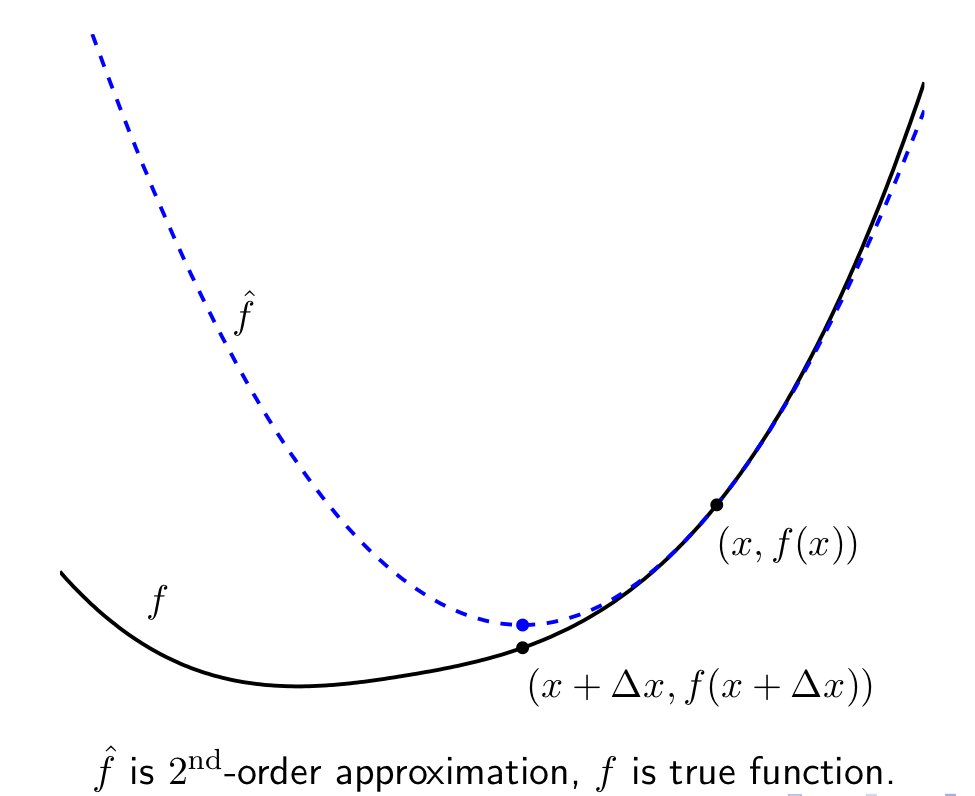
\includegraphics[width=5.5cm]{f1.png}
\end{center}
%\caption{visual representation of desired homotopy}
\label{12345678 figure name }%%%%%
\end{figure}

\end{frame}
%\frametitle{Newton's Method for Optimization}
%%%%%%%%%%%%%%%%%%%%%%%%%%%%%%%page 2 %%%%%%%%%%%%%%


 
 
\begin{frame}
\frametitle{Newton's Method in Higher Dimensions}
\begin{itemize}
       \item When $l$ is a function of multiple arguments
       \begin{center}
       $\theta_{n+1} = \theta_n - H^{-1} (\theta_n) \delta \ell(\theta_n)$
       \end{center}
       \item Calculating the inverse of $H$ is very time consuming 
        
   \end{itemize}
  \end{frame}
    




\begin{frame}
\begin{itemize}
    \item Pros 
    \begin{itemize}
    \item Converge quadratically
    \item Finds minima instead of general critical points
       \end{itemize}
        
            \item Cons 
               \begin{itemize}
               \item Newton's Method uses second partial derivatives, which may be complex to calculate
               \item Hessian matrix requires $O(n^3)$ operations to solve and $O(n^2)$ memory to store
               \item Newton's Method may diverge away from the root if the initial point is chosen poorly 
       \end{itemize}
          \end{itemize}
  \end{frame}





\begin{frame}
\frametitle{Newton's Method for Optimization}
\begin{itemize}
    \item  Because of the problems that Newton's Method has, We used Gradient Descent to minimize our cost function 
    \\
\begin{center}

  \end{center}
 
   \end{itemize}   
  \end{frame}
 



\begin{frame}
\frametitle{Gradient Descent}
\begin{itemize}

\item Having an estimate of $\delta \ell$, gradient of a function $\ell$ 
\item Decrease $\ell$ by a quantity along the direction of $\delta \ell$
  \begin{itemize}
  \item Direction
  \item Step size
  \end{itemize}
\item https://www.youtube.com/watch?v=GCvWD9zIF-s
\end{itemize}

\end{frame}



          

\begin{frame}
\frametitle{Quasi-Newton Method}

\begin{itemize}
\item Used when the problem size is big and the Hessian matrix is dense
\item Keeps "a rolling estimate" of $H(x)$ to solve this problem
\end{itemize}

  \end{frame}
  
% Newton's method as Iteratively Re-weighted Least Squares
% Frame 1
\begin{frame}
\frametitle{Newton's Method as Iteratively Re-weighted Least Squares}
\begin{itemize}
\item Recall, logistic regression model is a Bernoulli distribution with parameter $\sigmoid$:

\begin{equation}
\begin{split}
P(Y=y|X=\mathbf{x},\theta) &= \sigmoid^y (1 - \sigmoid)^{1-y}\\
&= \text{Ber}(y; \sigmoid)
\end{split}
\end{equation}

\item Again, logistic regression may be formulated as linear regression that best fits the \textit{log-odds}:
\begin{equation}
\begin{split}
\log \frac{P(Y=1|X=\mathbf{x},\theta)}{P(Y=0|X=\mathbf{x},\theta)} &= \log \frac{\sigmoid}{1 - \sigmoid}\\
&= \theta^T \mathbf{x}
\end{split}
\end{equation}

\end{itemize}
\end{frame}

% Frame 2
\begin{frame}
\frametitle{Newton's Method as Iteratively Re-weighted Least Squares}
\begin{itemize}
\item Linear regression is heavily affected by outliers - all observation variables may not have same precision of measurement (or \textit{variance}).
\item \textit{Weighted least squares} associates amount of $uncertainty$ at every point as a weight - large weights on points with \textit{high precision} or \textit{low variance} and vice-versa.
\item \textbf{Idea:} Multiply squared distance at each observation point by inverse of variance.
% Draw on board
\end{itemize}
\end{frame}

% Frame 3
\begin{frame}
\frametitle{Newton's Method as Iteratively Re-weighted Least Squares}
\begin{itemize}
\item Illustration:
\end{itemize}

\begin{figure}
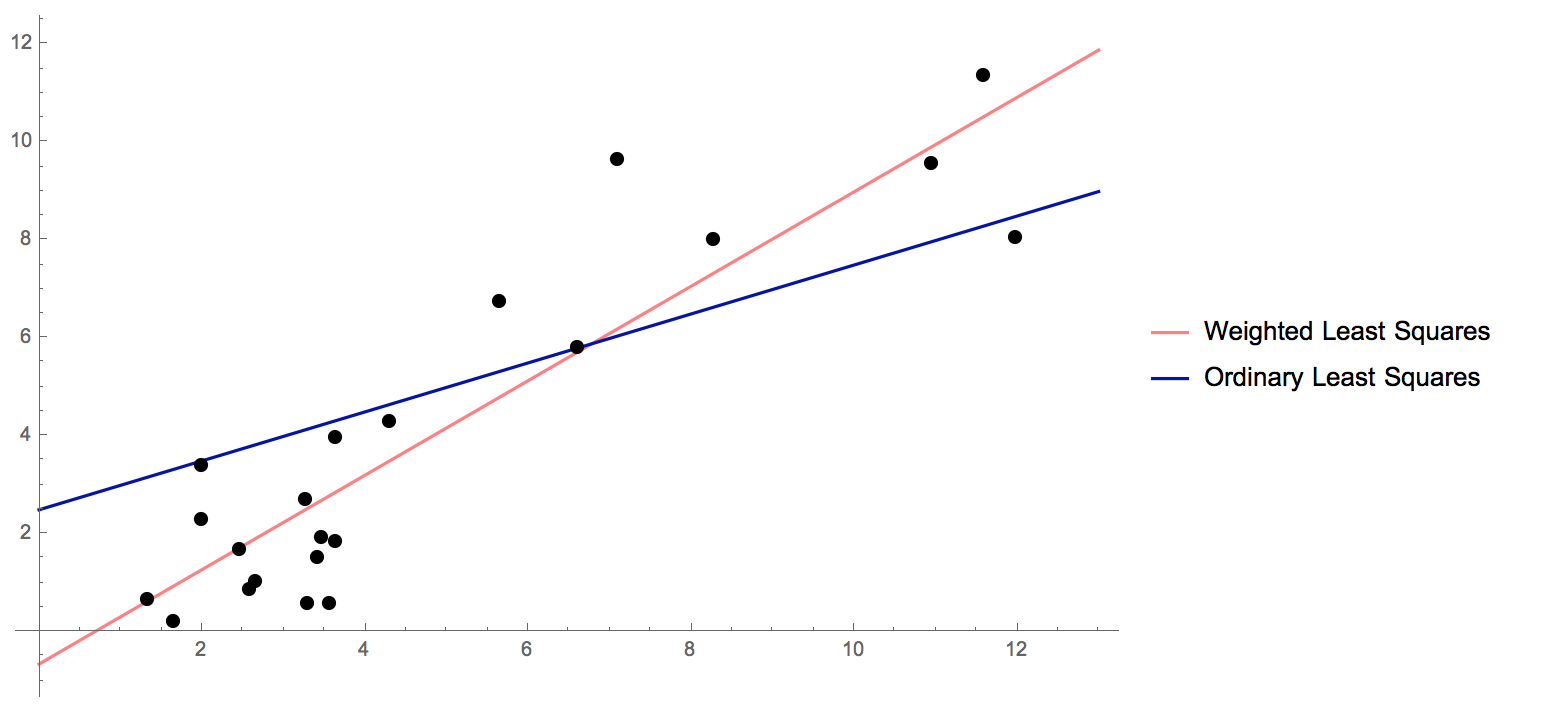
\includegraphics[scale = 0.4]{weightedLS}
\end{figure}
\end{frame}

% Frame 4
\begin{frame}
\frametitle{Newton's Method as Iteratively Re-weighted Least Squares}
\begin{itemize}
\item Loss function for weighted least squares regression (without regularization):
\begin{equation}
\mathcal{L(\theta)} = \sum_{i=1}^n \frac{1}{\text{Var}(y_i)}(y_i - \theta^T x_i)^2
\end{equation}
\item Least squares solution ($\text{Var}(y_i) = \text{const.})$:
\begin{equation}
\theta^* = (X^TX)^{-1}X^TY
\end{equation}
where $X = [x_1,...,x_n]^T, Y = [y_1,...,y_n]^T$.
\end{itemize}
\end{frame}

% Frame 5
\begin{frame}
\frametitle{Newton's Method as Iteratively Re-weighted Least Squares}
\begin{itemize}
\item \textit{Weighted} least squares solution:
\begin{equation}
\theta^* = (X^T WX)^{-1}X^T WY
\end{equation}
with $n \times n$ diagonal matrix $W_{ii} = \frac{1}{\text{Var}(y_i)}$
\item Variance of a Bernoulli distribution with parameter $p$ is $p(1-p)$. Hence, for logistic regression model,
\begin{equation}
W_{ii} = \frac{1}{\sigma (\theta^T x_i) (1 - \sigma (\theta^T x_i))}
\end{equation}
\end{itemize}
\end{frame}


% Frame 6
\begin{frame}
\frametitle{Newton's Method as Iteratively Re-weighted Least Squares}
\begin{itemize}
\item It can be shown that \textit{in expectation}, a step update by Newton's method on the logistic regression objective function is equivalent to reaching the weighted least-squares solution.
\item \textbf{Key reason}: Expected second derivative of the Bernoulli log-likelihood function is inversely proportional to the variance of the Bernoulli distribution (proof not shown).
\item However, not a single-step solution, as the weights themselves are functions of $\theta$ and the objective function is not quadratic.

%\item It can be shown that the Hessian matrix $H$ for the negative log-likelihood cost function is $H = X^T WX$ (and hence it is a convex function).
%\item Replacing $H$ and deriving the gradient from the weighted least-squares objective function, 
\end{itemize}
\end{frame}
  
  

%\end{document}